\documentclass{article}
\usepackage{amsmath}
\usepackage{graphicx}
\usepackage{url}
\usepackage{hyperref}
\hypersetup{
    colorlinks=true,
    linkcolor=blue,
    filecolor=magenta,      
    urlcolor=cyan,
}
\author{Kevin Lu, Travis You}
\title{Simulation and Inference for the Generalized Toilet Paper Problem}
\newtheorem{theorem}{Theorem}
\begin{document}
\maketitle
\begin{abstract}
This paper further investigates Knuth's toilet paper problem proposed in 1984 by studying the distribution of leftover toilet paper size in the non-empty roll when all other rolls empty with simulation. Shape, center, and variability of the distribution are found to be different at different $p$ (proportion of big-choosers), and the general trend is not affected by initial toilet paper size $n$ or the number of rolls present in the toilet stall. Inference for $p$ is carried out in the 2-roll case using Chebyshev's theorem and empirical bootstrapping method.
\end{abstract}
\section{Introduction}
In 1984, Knuth formulated a theoretical consideration for a ``toilet paper problem"\cite{Knuth1984}, which is a generalized matchbox problem from \cite{Feller}. Discussion of this problem can be generalized to other problems involving drawing out things from multiple containers.

Consider two types of people using a 2-roll toilet paper set: big-choosers and little-choosers. Big-choosers only uses toilet paper on the roll with more toilet paper and little-choosers only use toilet paper on the roll with less toilet paper. If both rolls have exactly the same amount of toilet paper, both types of people will randomly select a roll to use. Assume that all persons take 1 unit of toilet paper each time they use the restroom and that both rolls initially have $n$ units of toilet paper. If the amount of paper on the other roll when one roll is emptied is large, then the janitor would have plenty of time for replacement, but if that is not the case, people may run into problems.

Assume people enter the toilet independently at random, with proportion $p$ being big-choosers and proportion $q=1-p$ being little-choosers. Let $X$ be the random variable recording the number of paper left on one roll when the other roll first empties, Knuth showed that the expected value $E(X)$, denoted as $M_n(p)$, follows
\begin{equation}
    M_n(p) = n-\sum_{k=1}^{n-1} (n-k)c_k p^k q^{k-1}, 
    \label{Mnp}
\end{equation}
where $c_n = \binom{2n-2}{n-1}\frac{1}{n}$ is the catalan number. He has also given approximation of $M_n(p)$ for large $n$ as 
\begin{equation}
    M_n(p)=
    \begin{cases}
        \frac{q-p}{q}n+\frac{p}{q-p}+O(r^n) & \text{if }  p<1/2 \\
        \frac{p}{p-q} + O(r^n) & \text{if } p>1/2
    \end{cases}
    ,
    \label{limiting Mnp}
\end{equation}
where $r$ is any value greater than $4pq,$ which is smaller than $1$ for any $p \neq \frac{1}{2}$. The approximation in Eq.\eqref{limiting Mnp} works well when $|p-\frac{1}{2}|$ is at least of order $1/\sqrt{n}$. In that case, as $n$ is big, $O(r^n)$ is essentially 0. 

When $p$ is sufficiently close to $\frac{1}{2}$, the approximation in Eq.\eqref{limiting Mnp} does not work and $M_n(p)$ is better approximated by 
\begin{equation}
    M_n(p)=
    2\sqrt{\frac{n}{\pi}} - \frac{1}{4} \sqrt{\frac{1}{\pi n}} + O(n^{-3/2})
    \label{limiting Mnp equal}
\end{equation}

Therefore, when little-choosers predominate, $M_n(p)$ is of order $n$; when big-choosers predominate, $M_n(p)$ is of order $1$; when little-choosers and large-choosers are of similar number, $M_n(p)$ is of order $\sqrt{n}$. Moreover, there is a significant drop near $p=\frac{1}{2}$ for large $n$. 

In this paper, we're going to investigate further about the distribution of leftover amount $X$. Moreover, we're going to generalize the problem into a problem involving 3 and more rolls of toilet paper to test the claim that ``to solve the shortage of toilet paper when all other rolls empties, we just need to pile more rolls of toilet papers in the restroom.''
\section{2-Roll Simulation}
Random-walk simulation is made to study the distribution of leftover toilet paper X, as described in the following. Two integers $i$ and $k$ are initialized to the same value $n$, representing the initial size of toilet paper in each roll. A number is randomly generated from a uniform distribution of [0,1). If the number is less than $p$, then the larger number between $i$ and $k$ is subtracted by 1. If not, then the smaller number between $i$ and $k$ is subtracted by 1. If $i$ and $k$ are equal, then either of the two is randomly chosen to be subtracted by 1. This process of choosing a number and subtracting 1 is continued, each time with a new random number from [0,1), until one of $i$ and $k$ becomes 0. The value of the nonzero number is recorded as X, giving a 1-time random-walk simulation (code implementation in Appendix). 

To study the distribution of $X$, histogram of leftover paper size is drawn using 4000 simulations with $n=100$ at three different $p$, as shown in Fig.\ref{2roll-Histogram}.
\begin{figure}[ht]
    \centering
    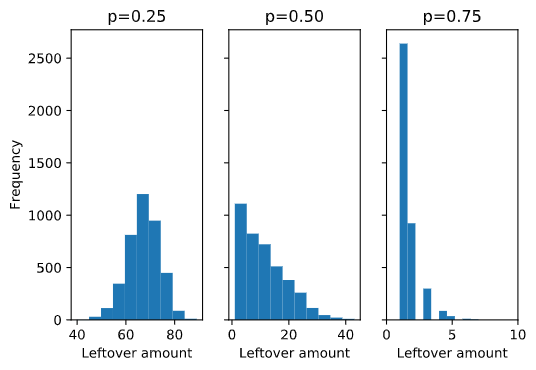
\includegraphics[width=10cm]{hist-2roll.png}
    \caption{Histogram of leftover paper size X with size 4000 at $p=0.25$ (left), $p=0.50$ (middle), and $p=0.75$ (right).}
    \label{2roll-Histogram}
\end{figure}
The shape of the distribution of leftover toilet paper size are different at different $p$, although all are unimodal. For $p<0.50$ (not too close to $0.50$), the distribution is approximately normal; for other cases, the distribution is skewed to the right and the right-skewness increases as $p$ increases. Center and variability will be discussed later using Fig.\ref{2roll-Mnp}.

In \cite{Knuth1984}, Knuth mainly discussed the expected value of leftover toilet paper size $M_n(p)$ and its approximate value when $n$ is large using Eq.\eqref{limiting Mnp} and Eq.\eqref{limiting Mnp equal}. As shown in Fig.\ref{2roll-approximation}, except for the horizontal line in the middle whose distance decreases as $n$ increases, the red and blue line are indistinguishable from each other. Therefore, the approximation in Eq.\eqref{limiting Mnp} and Eq.\eqref{limiting Mnp equal} work quite well at least for $n \geq 10$ for $p$ that deviates from $1/2$ with distance of order greater than $1/\sqrt{n}$. For $p$ that is sufficiently close to $1/2$, Eq.\eqref{limiting Mnp equal} provides a good estimation for the average value of $M_n(p)$ over this interval.
\begin{figure}[ht!]
    \centering
    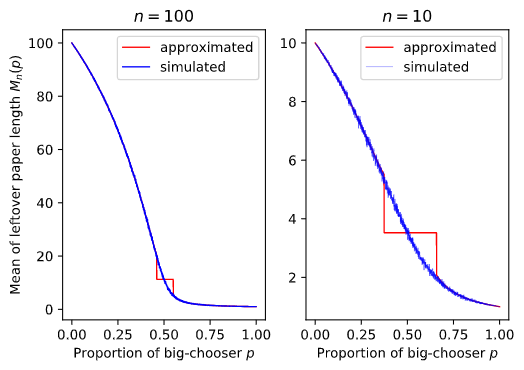
\includegraphics[width=10cm]{approxim-2roll.png}
    \caption{Comparison between approximated value in \cite{Knuth1984} and simulation result for computing expected value of leftover toilet paper size $M_n(p)$ at $n=100$ and $n=10$.}
    \label{2roll-approximation}
\end{figure} 

To further investigate center and variability of distribution for leftover toilet paper size, confidence band of $\bar{x} \pm 2s_x$ is drawn for three different initial toilet paper size $n$, where $\bar{x}$ is sample mean of $X$ and $s_x$ is sample standard deviation of $X$, as shown in Fig.\ref{2roll-Mnp}. The center of distribution (indicated by mean) initially starts from $O(n)$ and decreases gradually, then it decreases rapidly in the neighborhood of $p=0.5$ and quickly drops down to $O(1)$ after $p=0.6$. The variability, indicated by width of the error band, started small but grows quickly. After $p=0.6$, as in the case of center, the standard deviation drops down quickly. It should be noted that although skewness of distribution, as shown in Fig.\ref{2roll-Histogram}, makes mean a less accurate measure of center, the difference between curve showing mean of $X$ and median of $X$ at different $p$ is not significant. This is most likely because the skewness does not appear until $p \geq 1/2$, where the center has quickly descended to $O(1)$, making the difference less significant. In this paper, sample mean is preferred over median as a measure of center because exact mathematical expression for $M_n(p)$ and its accurate approximation Eq.\eqref{limiting Mnp} and Eq.\eqref{limiting Mnp equal} are handy. Moreover, it is easier to carry out inference using sample mean instead of median.
\begin{figure}[ht!]
    \centering
    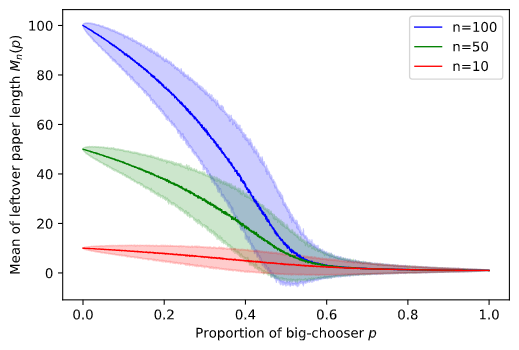
\includegraphics[width=10cm]{Mnp-2roll.png}
    \caption{Expected value of leftover toilet paper size $M_n(p)$ verses big-chooser proportion $p$ with confidence band of width 2 sample standard deviation at $n=10$, $n=50$, and $n=100$.}
    \label{2roll-Mnp}    
\end{figure}

\section{2-Roll Inference}
With knowledge of distribution of leftover toilet paper size, we are able to make inference of population proportion of big-choosers using sample data about leftover toilet paper size. By Eq.\eqref{Mnp}, population proportion of big chooser $p$ and population mean of leftover $M_n(p)$ follows a one-to-one map for $p \in [0,1]$. Therefore, we can first make inference about population mean of leftover $M_n(p)$ using confidence interval, which is directly related to the confidence interval for $p$. 

Suppose there are a lot of toilets in a building and we want to estimate population proportion of big-choosers in the building using a confidence interval. Assume that all stalls are equipped with 2-roll paper of length $100$ each. 5 stalls are randomly chosen from all stalls in the building, and the leftover amount of paper in the stalls are respectively 7, 10, 12, 13, 8. Thus distribution of $X$ has $\bar{x}=10$ and $s_x = 2.55$. Assume that there are more than 50 stalls in the building, which is reasonable for a large building with more than 10 toilets. 

Ideally, we would like to proceed with a 1-sample t-interval for population mean, which is subject to the condition that sample distribution of $X$ is approximately normal under small sample size. In this case, $\bar{x}$ is of $O(\sqrt{n})$, so from our previous knowledge, $p \approx 0.5$ and the sample distribution is skewed to the right. We could proceed with the 1-sample t-interval only if we know $p$ is significantly smaller than $0.5$ by observing, say, a large $\bar{x}=50$. If this is not the case, we must face the non-normality of sample distribution of $X$.

\subsection{Using Chebyshev's Theorem}
Chebyshev's theorem, which can be found in a typical statistical textbook like \cite{Freund}, states that 
\begin{theorem}
If $\mu$ and $\sigma$ ($\sigma \neq 0$)are the mean and standard deviation of a random variable $X$, then for any $k>0$,
\[
P(|x-\mu| < k\sigma) \geq 1-\frac{1}{k^2}.
\]
\label{Chebyshev's theorem}
\end{theorem}
Using Thm.\ref{Chebyshev's theorem}, at least $95\%$ of data falls in $4.47$ standard deviation from mean for any random variable. Using sample mean and standard error as point estimators, we can construct a confidence interval 
\begin{equation}
    \bar{x} \pm 4.47 \frac{s_x}{\sqrt{n}}
    =(4.90,15.10)
\end{equation}
and are at least $95\%$ confident that population mean of leftover toilet paper size in this building is between $4.90$ and $15.10$. Using endpoints of confidence interval for $\mu$ and the one-to-one map in Eq.\eqref{Mnp}, we are at least $95\%$ confident that population proportion of big-chooser in the building is between $0.481$ and $0.554$. 

\subsection{Using Empirical Bootstrapping}
It would be possible to use the empirical bootstrapping method\cite{bootstrap} to form a narrower confidence interval. The process is briefly summarized below (code implementation in Appendix). 

Using sampling with replacement, 10000 random samples of size 5 are drawn from the sample data of size 5. Mean of each random sample $\bar{x^*}$ is recorded to form a distribution of standard error $\delta^* = \bar{x^*}-\bar{x}$. The $2.5$th percentile $\delta^*_{.025}$ and the $97.5$th percentile $\delta^*_{.975}$ are calculated to form a $95$th confidence interval for population mean of leftover paper size
\begin{equation}
    (\bar{x}+\delta^*_{.025}, \bar{x}+\delta^*_{.975}) 
    = (8.0, 12.0).
\end{equation}
We are $95\%$ confident that population mean of leftover toilet paper size in this building is between $8.0$ and $12.0$. This is a narrower, thus more accurate, confidence interval compared to the one found with Chebyshev's theorem. Using endpoints of confidence interval for $\mu$ and the one-to-one map in Eq.\eqref{Mnp}, we are $95\%$ confident that population proportion of big-chooser in the building is between $0.496$ and $0.521$. 

\section{Multi-Roll Simulation}
Multi-roll problem is an extension of the 2-roll problem discussed by Knuth. Instead of considering the $M_n(p)$ when two rolls of toilet paper are presented, multi-roll problem investigates the $M_n(p)$ when $n$ rolls are presented, and how they differ from each other.

Random-walk simulations are written to simulate $M_n(p)$ at 3, 4, 5-roll scenarios. For example, to simulate the 3-roll problem, the program first generates and initializes three integers $i$, $j$, $k$ to the same $n$, which represents the initial number of toilet paper in each roll. Then, $p$ is compared to a random number $r$ generated from a uniform distribution of [0,1). If $r$ is less than $p$, the largest of $i$, $j$ and $k$ will be subtracted by 1. If $r$ is greater than $p$, the smallest of three variables will be subtracted by 1. If there are multiple variables with either the largest or the smallest value, the variable first generated will be subtracted by 1. The process from generating $r$ to subtracting 1 in one roll is looped until only one roll has toilet paper remained. The same procedure is used for 4-roll and 5-roll scenario except 4 or 5 variables are generated at first respectively. Finally, the $M_n(p)$ of this particular $p$ will be returned.

To answer the question that whether piling more rolls of toilet paper can solve the paper shortage, a $M_{100}(p)$ is simulated at 500 different $p$ values from $p=0$ to $p=1$ with the same step for 2, 3, 4, 5-rolls scenarios as shown in Fig.\ref{Mnp-compare}, where $\bar{x}$ is the sample mean for $X$. Before $p=0.6$, four centers of distributions gradually decreases, starting from $O(n)$. After $p=0.6$, four centers of distribution converges, approaching $O(1)$. As the number of rolls increases, the curve becomes more linear and eventually converges to a roughly linear function for $p \in [0 ,0.5]$. This makes every $M_{100}(p)$ for an $n$-roll case smaller than an $m$-roll case where $m<n$ before $p=0.6$. Thus, piling more rolls will result in a worse situation that leftover paper are less, rather than increasing the number. This phenomenon can be explained by viewing n-roll case as 2-roll case with one roll of the least paper and multiple rolls of approximately the same amount of paper. As smaller-choosers only choose the roll with the least paper, one roll will always has the least paper, if not the same as other rolls. However, the behavior of big-chooser will create multiple rolls with approximately the same amount of paper. When $x$-roll case starts, it starts from $O(n_1)$, where $n_1$ represents the initial amount of toilet paper for each roll. After the least-paper roll is depleted, the case then becomes another "2-roll case" with $x-1$ rolls starting from $O(n_2)$, where $n_2$ represents the total amount of toilet paper for each roll after the depletion of the least-paper roll. Comparing to a standard 2-roll case that always keeps its order at $n_1$ before the lower bound of the interval calculated from Eq.\eqref{limiting Mnp equal}, the order of n-roll case is always decreasing as more rolls are depleted.
\begin{figure}[hb!]
    \centering
    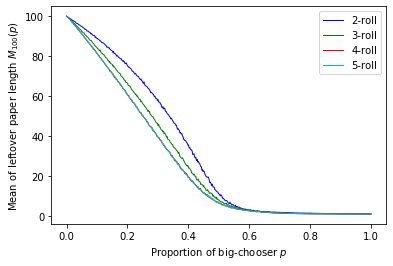
\includegraphics[width=10cm]{2345roll-comparison.png}
    \caption{Expected value of leftover toilet paper size $M_n(p)$ verses big-chooser proportion $p$ for 2-roll, 3-roll, 4-roll, and 5-roll cases.}
    \label{Mnp-compare}
\end{figure}

\section{Conclusion}
Random-walk simulation is used to investigate the distribution of $X$ (leftover toilet paper size in the non-empty roll when all other rolls empty) in the toilet paper problem\cite{Knuth1984}. Distribution of $X$ is normal when $p$ is noticeably smaller than $0.5$ and is skewed to the right in other cases. $E(X)$ as a function of $p$ are quite similar for different roll numbers, so piling more rolls of toilet paper does not solve the shortage of toilet paper in the non-empty roll, if not making the situation worse. Knuth's approximation formula for $E(X)$ in 2-roll case is very accurate for $p$ not too close to $0.5$. Variability of $X$ is small for small and large $p$ and large otherwise. Chebyshev's theorem and bootstrapping can be used to make inference about $p$ when sample distribution of $X$ is obtained, and the method using bootstrapping is more accurate. Further research may focus on exactly calculating standard deviation of $X$ in 2-roll case and describing exact distribution of $X$ in all cases, which would enable the use of parametric bootstrapping and increase accuracy of inference. 

\section{Appendix}
Code implementation for computing mentioned in this paper can be found at \url{https://github.com/Kevin-Luyu/Semester2-Final-Project}. 
\bibliographystyle{plain}
\bibliography{MyCollection.bib}
\end{document}